\chapter{Perancangan}
\label{chap:perancangan}

Pada bab ini akan dijelaskan perancangan program yang dibuat pada penelitian ini. Perancangan terdiri dari masukan program ,aktivitas sistem.

\section{Rancangan Antarmuka}

\subsection{Rancangan Antarmuka Formulir Data Baru Umat}

\begin{figure}[H]
	\centering
	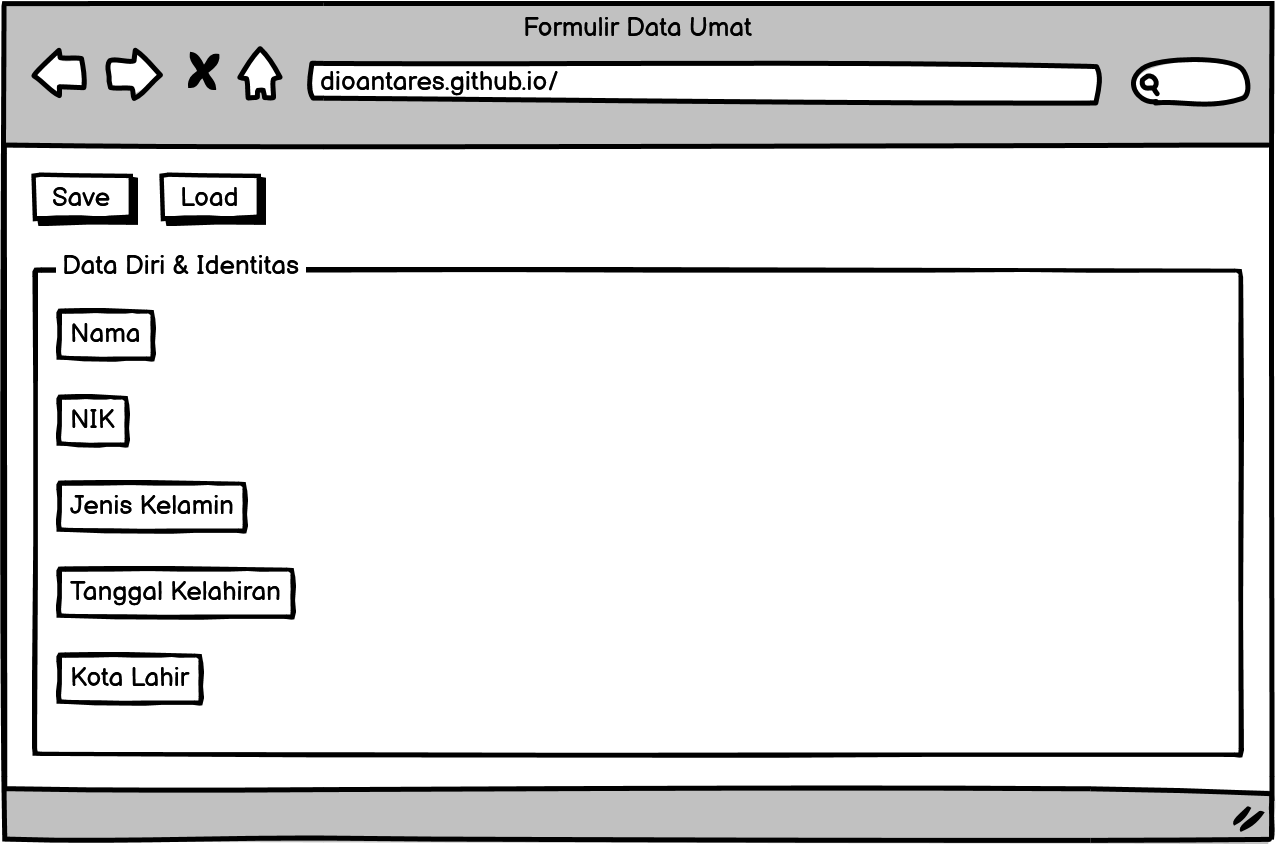
\includegraphics[scale=0.7]{Gambar/mockUpWebsite.png}
	\caption{Rancangan antarmuka halaman Formulir Data Umat} 
	\label{fig:formDataUmat}
\end{figure}

Seluruh fitur akan diimplementasikan pada halaman website yang berisikan formulir data umat. Gambar \ref{fig:formDataUmat} menunjukkan rancangan antarmuka halaman formulir data umat. Pada halaman formulir data umat sudah terdapat fitur save, load, submit, dan akan ada  beberapa perubahan pada rancangan baru formulir data baru umat, contoh perubahan tersebut adalah : 

\begin{enumerate}
	\item Halam formulir dapat dibuka di mobile dengan baik \textit{(responsive design)}.
	\item Memunculkan keyboard yang tepat untuk input tertentu (contoh: nomor telepon menggunakan keypad)
	\item Menyimpan data secara otomatis di penyimpanan lokal, sehingga saat dibuka kembali, umat dapat melanjutkan pengisian. Fitur ini telah diimplementasikan pada tombol \textit{save} dan \textit{load}.
\end{enumerate}

\newpage

\subsection{Fitur Save}

\begin{figure}[H]
	\centering
	
\includegraphics[scale=0.7]{Gambar/fiturSave.png}
	\caption{Fitur save pada website formulir data umat} 
	\label{fig:fiturSave}
\end{figure}

Fitur tombol \textit{Save} pada halaman ini berfungsi untuk menyimpan data yang telah diisi oleh umat. Formulir ini berisikan cukup banyak \textit{field} untuk diisi, sehingga apabila formulir ini tertutup atau umat akan melanjutkannya nanti, data akan tersimpan pada \textit{cookies}.

\subsection{Fitur Load}

\begin{figure}[H]
	\centering
	
\includegraphics[scale=0.7]{Gambar/fiturLoad.png}
	\caption{Fitur load pada website formulir data umat} 
	\label{fig:fiturLoad}
\end{figure}

Fitur tombol \textit{Load} pada halaman ini berfungsi untuk mengisi data secara otomatis yang telah diisi oleh umat, fitur ini akan berjalan apabila sebelumnya umat sudah mengisi data lalu menggunakan fitur \textit{Save}. Tujuan utama dari fitur \textit{Load} ini adalah untuk mengambil data lalu mengisikannya secara otomatis pada field yang telah tersediah, sehingga apabila umat melanjutkan mengisi formulir, waktu yang diperlukan tidak perlu lama karena data akan diambil dari \textit{cookies}.

\subsection{Fitur Submit}

\begin{figure}[H]
	\centering
	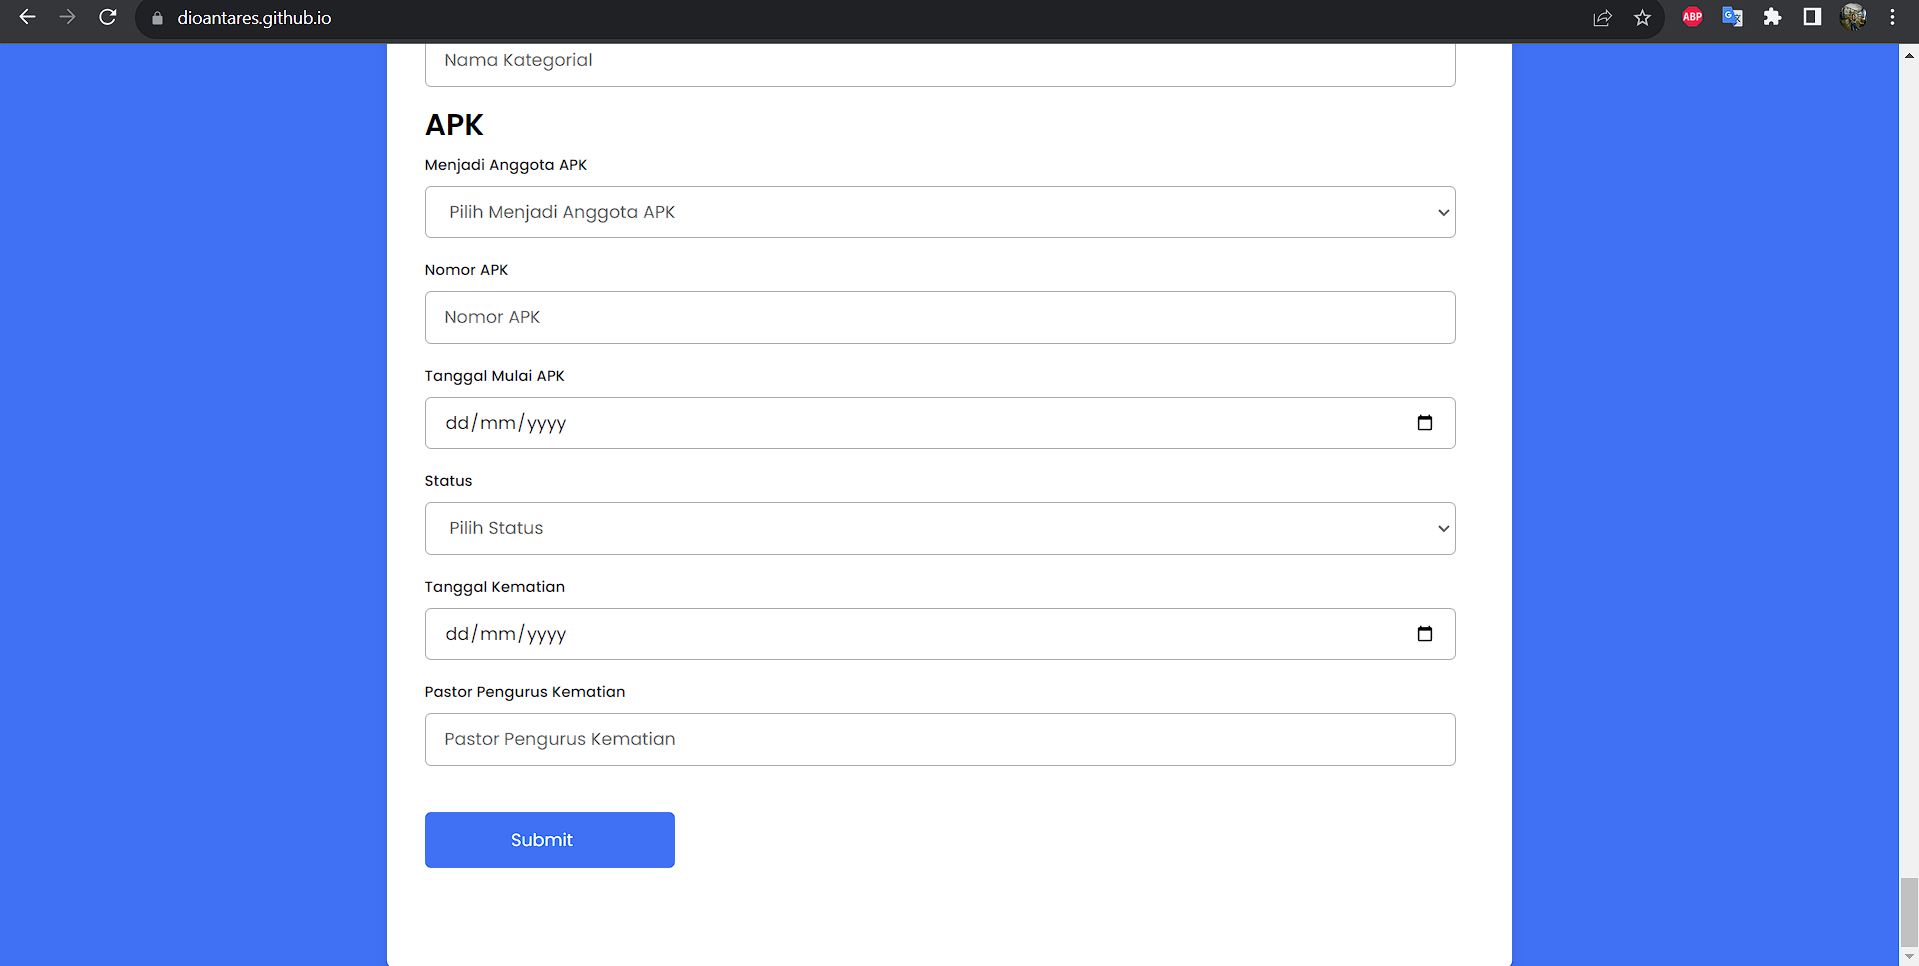
\includegraphics[scale=0.7]{Gambar/fiturSubmit.png}
	\caption{Fitur submit pada website formulir data umat} 
	\label{fig:fiturSubmit}
\end{figure}

Fitur tombol \textit{Submit} pada halaman ini berfungsi untuk mengubah data yang telah terisi menjadi \textit{qr code}. Penggunaan fitur ini bertujuan agar \textit{qr code} dapat dipindai oleh admin dan dimasukan ke sistem SIMU.




